\section{Langkah-Langkah Percobaan}

\subsection{Persiapan Praktikum}
\begin{enumerate}
    \item Membuka aplikasi Visual Studio Code dengan ekstensi PlatformIO yang telah terinstal.
    \item Membuat proyek baru bernama \texttt{modul2-sensor-aktuator} dengan konfigurasi board \textbf{Espressif ESP32 Dev Module} dan framework \textbf{Arduino}.
    \item Mengatur kecepatan komunikasi serial pada berkas \texttt{platformio.ini} menjadi \texttt{monitor\_speed = 115200}, serta menambahkan pustaka \texttt{madhephaestus/ESP32Servo@\^{}3.0.0} khusus untuk percobaan motor servo.
    \item Memastikan catu daya eksternal dalam keadaan mati (\textit{OFF}) dan melepas rangkaian percobaan sebelumnya sebelum merakit rangkaian percobaan berikutnya.
\end{enumerate}

\subsection{Percobaan 1: Sensor Resistif, Kapasitif, dan Induktif}
\begin{enumerate}
    \item Menghubungkan modul joystick KY-023 ke ESP32: pin \texttt{VRx} ke \texttt{GPIO 34}, \texttt{VRy} ke \texttt{GPIO 35}, \texttt{SW} ke \texttt{GPIO 27}, serta \texttt{VCC} dan \texttt{GND} ke pin \texttt{3.3V} dan \texttt{GND} ESP32.
    \item Menghubungkan pin \texttt{OUT} modul \textit{touch sensor} TTP223 ke \texttt{GPIO 4} serta pin \texttt{DO/OUT} sensor \textit{hall effect} ke \texttt{GPIO 26}, dengan suplai \texttt{3.3V} dan \texttt{GND}.
    \item Menulis kode pembacaan ADC dan input digital pada \texttt{src/main.cpp}, lalu melakukan proses \textit{Build} dan \textit{Upload} ke ESP32.
    \item Membuka Serial Monitor pada baud rate \texttt{115200}, kemudian menggerakkan serta menekan tuas joystick, menyentuh pad TTP223, dan mendekatkan magnet ke sensor \textit{hall effect} untuk mengamati perubahan nilai pada Serial Monitor.
\end{enumerate}

\subsection{Percobaan 2: Sensor Ultrasonik dan IR Obstacle}
\begin{enumerate}
    \item Menghubungkan sensor ultrasonik HC-SR04 ke ESP32: pin \texttt{Trig} ke \texttt{GPIO 5}, \texttt{Echo} ke \texttt{GPIO 18}, \texttt{VCC} ke \texttt{5V}, dan \texttt{GND} ke \texttt{GND}.
    \item Menghubungkan pin \texttt{OUT} sensor IR \textit{obstacle} ke \texttt{GPIO 19} serta \texttt{VCC/GND} ke \texttt{3.3V/GND} ESP32.
    \item Mengunggah kode program pembacaan durasi pulsa pantulan ultrasonik dan status digital IR ke ESP32.
    \item Membuka Serial Monitor (\texttt{115200} baud), lalu mendekatkan dan menjauhkan objek di depan kedua sensor untuk mengamati hasil pengukuran jarak (cm) dan status deteksi halangan.
\end{enumerate}

\subsection{Percobaan 3: Aktuator Motor DC}
\begin{enumerate}
    \item Menghubungkan joystick KY-023 (\texttt{VRx} ke \texttt{GPIO 34}, \texttt{SW} ke \texttt{GPIO 27}, \texttt{VCC} ke \texttt{5V}, dan \texttt{GND} ke \texttt{GND}) sebagai pengendali interaktif.
    \item Melepas jumper \texttt{ENA} pada driver L298N, lalu menghubungkan \texttt{ENA} ke \texttt{GPIO 25}, \texttt{IN1} ke \texttt{GPIO 26}, dan \texttt{IN2} ke \texttt{GPIO 33}.
    \item Menghubungkan kabel motor DC (\texttt{M1} dan \texttt{M2}) ke terminal \texttt{OUT1} dan \texttt{OUT2} driver L298N, serta menyambungkan catu daya eksternal \texttt{12V} ke terminal \texttt{+12V} dan menyatukan jalur \texttt{GND} catu daya, L298N, dan ESP32 (\textit{common ground}).
    \item Mengunggah kode kontrol PWM ke ESP32 dan membuka Serial Monitor (\texttt{115200} baud).
    \item Menggeser tuas joystick ke kiri dan ke kanan untuk mengamati perubahan arah serta kecepatan putar motor DC, lalu menekan tombol \texttt{SW} untuk menguji fungsi \textit{stop} darurat.
\end{enumerate}

\subsection{Percobaan 4: Aktuator Motor Stepper}
\begin{enumerate}
    \item Menghubungkan pin \texttt{IN1}, \texttt{IN2}, \texttt{IN3}, dan \texttt{IN4} pada modul driver ULN2003 masing-masing ke \texttt{GPIO 16}, \texttt{GPIO 17}, \texttt{GPIO 18}, dan \texttt{GPIO 19} ESP32.
    \item Memasang konektor motor stepper 28BYJ-48 ke modul driver ULN2003 serta menghubungkan catu daya eksternal dengan \textit{common ground} ke ESP32.
    \item Mengunggah kode pengendalian 8-langkah (\textit{half-step}) untuk rotasi $90^\circ$ (1024 \textit{step}) dengan jeda 0,5 detik.
    \item Mengamati gerakan poros motor stepper dan kesesuaian statusnya pada Serial Monitor (\texttt{115200} baud).
\end{enumerate}

\subsection{Percobaan 5: Aktuator Motor Servo}
\begin{enumerate}
    \item Menghubungkan kabel sinyal motor servo ke \texttt{GPIO 13}, kabel daya (\texttt{VCC}) ke pin \texttt{5V} ESP32, dan kabel \texttt{GND} ke \texttt{GND} ESP32.
    \item Mengunggah kode program yang menggunakan pustaka \texttt{ESP32Servo} pada frekuensi \texttt{50 Hz} ke ESP32.
    \item Membuka Serial Monitor (\texttt{115200} baud) dan mengamati pergerakan lengan servo secara bolak-balik antara sudut $180^\circ$ (CW) dan $0^\circ$ (CCW) dengan jeda 0,5 detik.
\end{enumerate}

\subsection{Percobaan 6: Aktuator ESC dan Motor Brushless (BLDC)}
\begin{enumerate}
    \item Memastikan sakelar catu daya eksternal dalam kondisi mati (\textit{OFF}) dan motor BLDC tidak terpasang baling-baling (\textit{propeller}).
    \item Menghubungkan kabel sinyal ESC ke \texttt{GPIO 25}, menyatukan jalur \texttt{GND} ESC dengan \texttt{GND} ESP32, membiarkan kabel merah BEC tidak terhubung ke pin \texttt{3.3V} ESP32, serta menyambungkan tiga kabel fasa output ESC ke motor BLDC.
    \item Mengunggah kode pembangkit sinyal PWM LEDC \texttt{50 Hz} resolusi 16-bit ke ESP32, kemudian mencabut kabel USB dan memastikan jalur \texttt{VIN} serta \texttt{GND} terpasang sesuai skema modul.
    \item Menyalakan daya eksternal tepat pada jeda waktu \textit{arming} 5 detik (saat sinyal minimum \texttt{1000 $\mu$s} dikirim), lalu mengamati motor BLDC berputar naik bertahap dari PWM \texttt{0} hingga \texttt{128} dan turun kembali ke \texttt{0}.
\end{enumerate}

\section{Analisis Hasil Percobaan}

\subsection{Percobaan 1: Sensor Resistif, Kapasitif, dan Induktif}
Pengujian ketiga sensor pada rangkaian terpadu menghasilkan pembacaan nilai analog dan logika digital pada Serial Monitor sebagai berikut:
\begin{itemize}
    \item \textbf{Sensor Resistif (Joystick KY-023):} Pada kondisi tuas diam (netral), nilai ADC 12-bit terbaca pada kisaran \texttt{VRx = 2798--2861} dan \texttt{VRy = 2896--2950}, tidak tepat berada pada titik tengah teoritis \texttt{2048}. Saat tuas digeser ke batas ekstrem, nilai pembacaan mencapai batas bawah \texttt{VRx = 0} (\texttt{VRy = 3655--3702}) dan batas atas \texttt{VRx = 4095} serta \texttt{VRy = 4095}. Tombol tekan \texttt{SW} terbaca \texttt{idle} saat dilepas dan berubah menjadi \texttt{DITEKAN} saat ditekan, sesuai konfigurasi \texttt{INPUT\_PULLUP} dengan logika \textit{active-low}.
    \item \textbf{Sensor Kapasitif (TTP223):} Status pada Serial Monitor berubah dari \texttt{idle} menjadi \texttt{TERSENTUH} (disertai menyalanya LED indikator modul) tepat ketika jari menyentuh permukaan pad. Hal ini sesuai dengan teori bahwa IC TTP223 memiliki rangkaian pembanding ambang batas internal sehingga menghasilkan keluaran digital \textit{active-high} siap pakai tanpa memerlukan kalibrasi nilai mentah seperti fungsi \texttt{touchRead()}.
    \item \textbf{Sensor Induktif (\textit{Hall Effect}):} Saat tidak ada sumber medan magnet di sekitar sensor, status terbaca \texttt{idle}. Ketika magnet kecil didekatkan ke permukaan sensor, status langsung berubah menjadi \texttt{MAGNET TERDETEKSI} dengan logika \textit{active-low} akibat perubahan fluks medan magnet yang mengenai elemen Hall.
\end{itemize}

\textbf{Faktor yang Memengaruhi Hasil:} Pergeseran titik netral joystick dari nilai ideal \texttt{2048} ke kisaran \texttt{2840--2950} serta fluktuasi kecil ($\pm 30\text{--}60$ unit ADC) dipengaruhi oleh toleransi mekanis pegas dan potensiometer di dalam modul KY-023, non-linearitas karakteristik ADC ESP32, serta \textit{noise} kontak pada kabel jumper dan \textit{breadboard}. Temuan ini membuktikan perlunya penerapan \textit{dead zone} agar aktuator tidak bergerak sendiri saat tuas tidak disentuh.

\subsection{Percobaan 2: Sensor Ultrasonik HC-SR04 dan IR Obstacle}
Hasil pengujian sensor berbasis akustik dan optik menunjukkan karakteristik deteksi yang berbeda terhadap posisi objek:
\begin{itemize}
    \item \textbf{Sensor Ultrasonik (HC-SR04):} Pengukuran jarak menggunakan persamaan $d = \frac{t \times 0,0343}{2}$ mampu menampilkan jarak objek secara kuantitatif pada rentang menengah, seperti \texttt{3,6 cm}, \texttt{7,1 cm}, \texttt{7,8 cm}, \texttt{8,1 cm}, \texttt{16,8 cm}, hingga \texttt{36,8 cm}. Ketika objek dijauhkan keluar jangkauan atau didekatkan terlalu rapat ke transduser ($< 2\text{--}3\text{ cm}$), fungsi \texttt{pulseIn()} mencapai batas \textit{timeout} \texttt{30000 us} dan menampilkan \texttt{Jarak: tidak ada objek}.
    \item \textbf{Sensor IR \textit{Obstacle}:} Pada jarak menengah (\texttt{7,8--36,8 cm}), sensor IR masih berstatus \texttt{idle}. Status baru berubah menjadi \texttt{TERDETEKSI} (\textit{active-low}) saat jari didekatkan tepat di depan LED pemancar dan fotodioda penerima inframerah.
\end{itemize}

\textbf{Faktor yang Memengaruhi Hasil:} Sensor HC-SR04 memiliki \textit{blind zone} pada jarak sangat dekat karena transduser penerima masih bergetar sesaat setelah memancarkan pulsa, serta sempat muncul lonjakan pembacaan sesaat sebesar \texttt{231,0 cm} akibat pantulan gema dari benda lain di sekitar meja praktikum (\textit{multipath reflection}). Sebaliknya, sensor IR \textit{obstacle} sangat responsif untuk deteksi biner jarak dekat, tetapi jarak ambang deteksinya bergantung pada pengaturan potensiometer sensitivitas modul dan daya pantul (reflektansi) permukaan objek.

\subsection{Percobaan 3: Aktuator Motor DC}
Pengendalian motor DC JGA25-370 melalui driver L298N dan joystick KY-023 berjalan sesuai prinsip modulasi lebar pulsa (PWM):
\begin{itemize}
    \item \textbf{Kontrol Arah dan Kecepatan Proporsional:} Saat tuas joystick digeser penuh ke satu sisi, Serial Monitor menampilkan \texttt{Motor: MUNDUR, PWM = 255} dan poros motor berputar pada kecepatan maksimum. Saat digeser penuh ke arah berlawanan, keluaran berubah menjadi \texttt{Motor: MAJU, PWM = 254} dengan arah putar berbalik. Pada pergeseran tuas sebagian, terbaca nilai menengah \texttt{Motor: MAJU, PWM = 64--65} dengan kecepatan putar motor yang melambat secara proporsional.
    \item \textbf{Fungsi \textit{Dead Zone} dan \textit{Stop} Darurat:} Saat tuas dilepas ke posisi netral (\texttt{abs(deviation) < 300}), sinyal PWM bernilai \texttt{0} sehingga motor berhenti. Penekanan tombol \texttt{SW} langsung mengaktifkan prioritas \textit{stop} darurat yang menghentikan putaran motor seketika.
\end{itemize}

\textbf{Faktor yang Memengaruhi Hasil:} Hasil ini mengonfirmasi teori bahwa pada motor DC, \textit{duty cycle} sinyal PWM mengatur tegangan rata-rata yang menentukan kecepatan putar, sedangkan kombinasi logika digital \texttt{IN1} dan \texttt{IN2} pada driver L298N membalik polaritas arah arus motor. Keberhasilan kontrol sangat bergantung pada penyatuan jalur ground (\textit{common ground}) antara catu daya eksternal \texttt{12 V}, driver L298N, dan ESP32, serta kesesuaian kalibrasi titik tengah (\texttt{JOY\_CENTER}) terhadap toleransi potensiometer joystick yang digunakan.

\subsection{Percobaan 4: Aktuator Motor Stepper}
Pengujian motor stepper unipolar 28BYJ-48 melalui driver ULN2003 menghasilkan gerakan diskret yang terukur:
\begin{itemize}
    \item \textbf{Presisi Sudut Putaran:} Serial Monitor menampilkan siklus \texttt{Motor berputar 90 derajat} diikuti \texttt{Motor berhenti 0.5 detik} secara berulang. Pengamatan pada penanda poros menunjukkan poros motor berputar konsisten sebesar seperempat putaran ($90^\circ$) pada setiap siklus.
    \item \textbf{Kesesuaian Waktu Siklus:} Dengan spesifikasi \texttt{4096 step} per putaran penuh ($360^\circ$), rotasi $90^\circ$ mengeksekusi tepat \texttt{1024 step} pola \textit{half-step} 8 langkah. Dengan jeda antar-langkah \texttt{STEP\_DELAY\_US = 2000 us}, satu kali rotasi $90^\circ$ membutuhkan waktu $1024 \times 2\text{ ms} \approx 2,05\text{ detik}$, diikuti jeda diam selama \texttt{500 ms}.
\end{itemize}

\textbf{Faktor yang Memengaruhi Hasil:} Ketepatan urutan logika 4-fasa pada pin \texttt{IN1--IN4} menentukan kelancaran medan magnet putar pada stator; kesalahan urutan kabel akan menyebabkan poros motor hanya bergetar tanpa berputar. Selain itu, pemanggilan fungsi \texttt{stopMotor()} yang memutus arus seluruh koil saat jeda efektif mencegah pemanasan berlebih (\textit{overheating}) pada motor, meskipun menghilangkan torsi penahan (\textit{holding torque}) selama motor berhenti.

\subsection{Percobaan 5: Aktuator Motor Servo}
Pengendalian motor servo menggunakan pustaka \texttt{ESP32Servo} menunjukkan kesesuaian antara lebar pulsa sinyal PWM dengan posisi sudut lengan servo:
\begin{itemize}
    \item \textbf{Gerak Bolak-Balik Sudut Target:} Serial Monitor menampilkan pesan \texttt{Servo bergerak CCW ke 0 derajat} dan \texttt{Servo bergerak CW ke 180 derajat} yang masing-masing diikuti status \texttt{Gerakan selesai (estimasi)} serta \texttt{Berhenti selama 0.5 detik}. Secara fisik, lengan servo bergerak akurat bolak-balik menuju kedua titik sudut target tersebut.
    \item \textbf{Interpretasi Lebar Pulsa:} Hasil ini membuktikan bahwa berbeda dari motor DC yang membaca nilai rata-rata tegangan, rangkaian kontrol internal servo menerjemahkan lebar pulsa spesifik (\texttt{500 us} untuk $0^\circ$ dan \texttt{2400 us} untuk $180^\circ$) dalam periode tetap \texttt{20 ms} (\texttt{50 Hz}) menjadi posisi sudut absolut.
\end{itemize}

\textbf{Faktor yang Memengaruhi Hasil:} Karena motor servo standar tidak mengirimkan sinyal umpan balik posisi kembali ke mikrokontroler (\textit{open-loop} di sisi ESP32), akurasi jeda gerakan sangat bergantung pada penetapan waktu tunda estimasi (\texttt{MOVE\_TIME\_MS} sebesar \texttt{500 ms} pada kode uji) agar lengan servo benar-benar selesai bergerak sebelum perintah berikutnya dikirimkan, serta kestabilan suplai tegangan \texttt{5 V} untuk mencegah penurunan tegangan sesaat saat motor mulai bergerak.

\subsection{Percobaan 6: Aktuator ESC dan Motor Brushless (BLDC)}
Pengujian motor brushless (BLDC) melalui Electronic Speed Controller (ESC) \texttt{20 A} membuktikan mekanisme komutasi elektronik dan prosedur keamanan \textit{arming}:
\begin{itemize}
    \item \textbf{Proses \textit{Arming} dan Kontrol LEDC:} Sinyal PWM \texttt{50 Hz} beresolusi 16-bit (\texttt{0--65535}) dibangkitkan langsung melalui peripheral \textit{hardware} \texttt{LEDC} tanpa pustaka \texttt{ESP32Servo}. Ketika sinyal throttle minimum \texttt{1000 us} (\texttt{PWM = 0}) dikirimkan terlebih dahulu dan catu daya eksternal dinyalakan dalam rentang waktu 5 detik, ESC mengeluarkan bunyi \textit{beep} yang menandakan proses \textit{arming} berhasil.
    \item \textbf{Respons Kecepatan Bertahap:} Setelah \textit{arming} selesai, putaran motor BLDC meningkat secara halus dari posisi diam (\texttt{PWM = 0}) hingga kecepatan menengah (\texttt{PWM = 128} atau lebar pulsa sekitar \texttt{1502 us}, setara 50\% throttle), bertahan selama \texttt{0,5 detik}, lalu melambat kembali secara bertahap hingga berhenti.
\end{itemize}

\textbf{Faktor yang Memengaruhi Hasil:} Urutan penyalaan daya menjadi faktor paling menentukan pada percobaan ini. Apabila catu daya ESC terlambat dinyalakan setelah jeda 5 detik berakhir—ketika program sudah memasuki \texttt{loop()} dan menaikkan nilai PWM di atas \texttt{1000 us}—ESC akan menolak melakukan \textit{arming} sebagai fitur pengaman agar motor tidak berputar mendadak. Selain itu, pelepasan baling-baling (\textit{propeller}) dan pembatasan uji hingga nilai \texttt{PWM = 128} memastikan pengujian berlangsung aman dan stabil di atas papan praktikum.

\section{Hasil Tugas Modul}

\subsection{Simulasi Motor Stepper Sebagai Jam Analog}
Simulasi dirancang menggunakan mikrokontroler ESP32 dengan tiga buah motor stepper bipolar ($200$ step per putaran atau $1,8^\circ$ per step) yang masing-masing dikendalikan melalui driver A4988 pada platform Wokwi. Setiap motor merepresentasikan jarum milidetik, detik, dan menit pada jam analog. Agar ketiga motor dapat berputar secara bersamaan tanpa saling menghambat, pembangkitan pulsa STEP diatur menggunakan pencacah waktu berbasis fungsi \texttt{micros()}.

\begin{figure}[htbp]
    \centering
    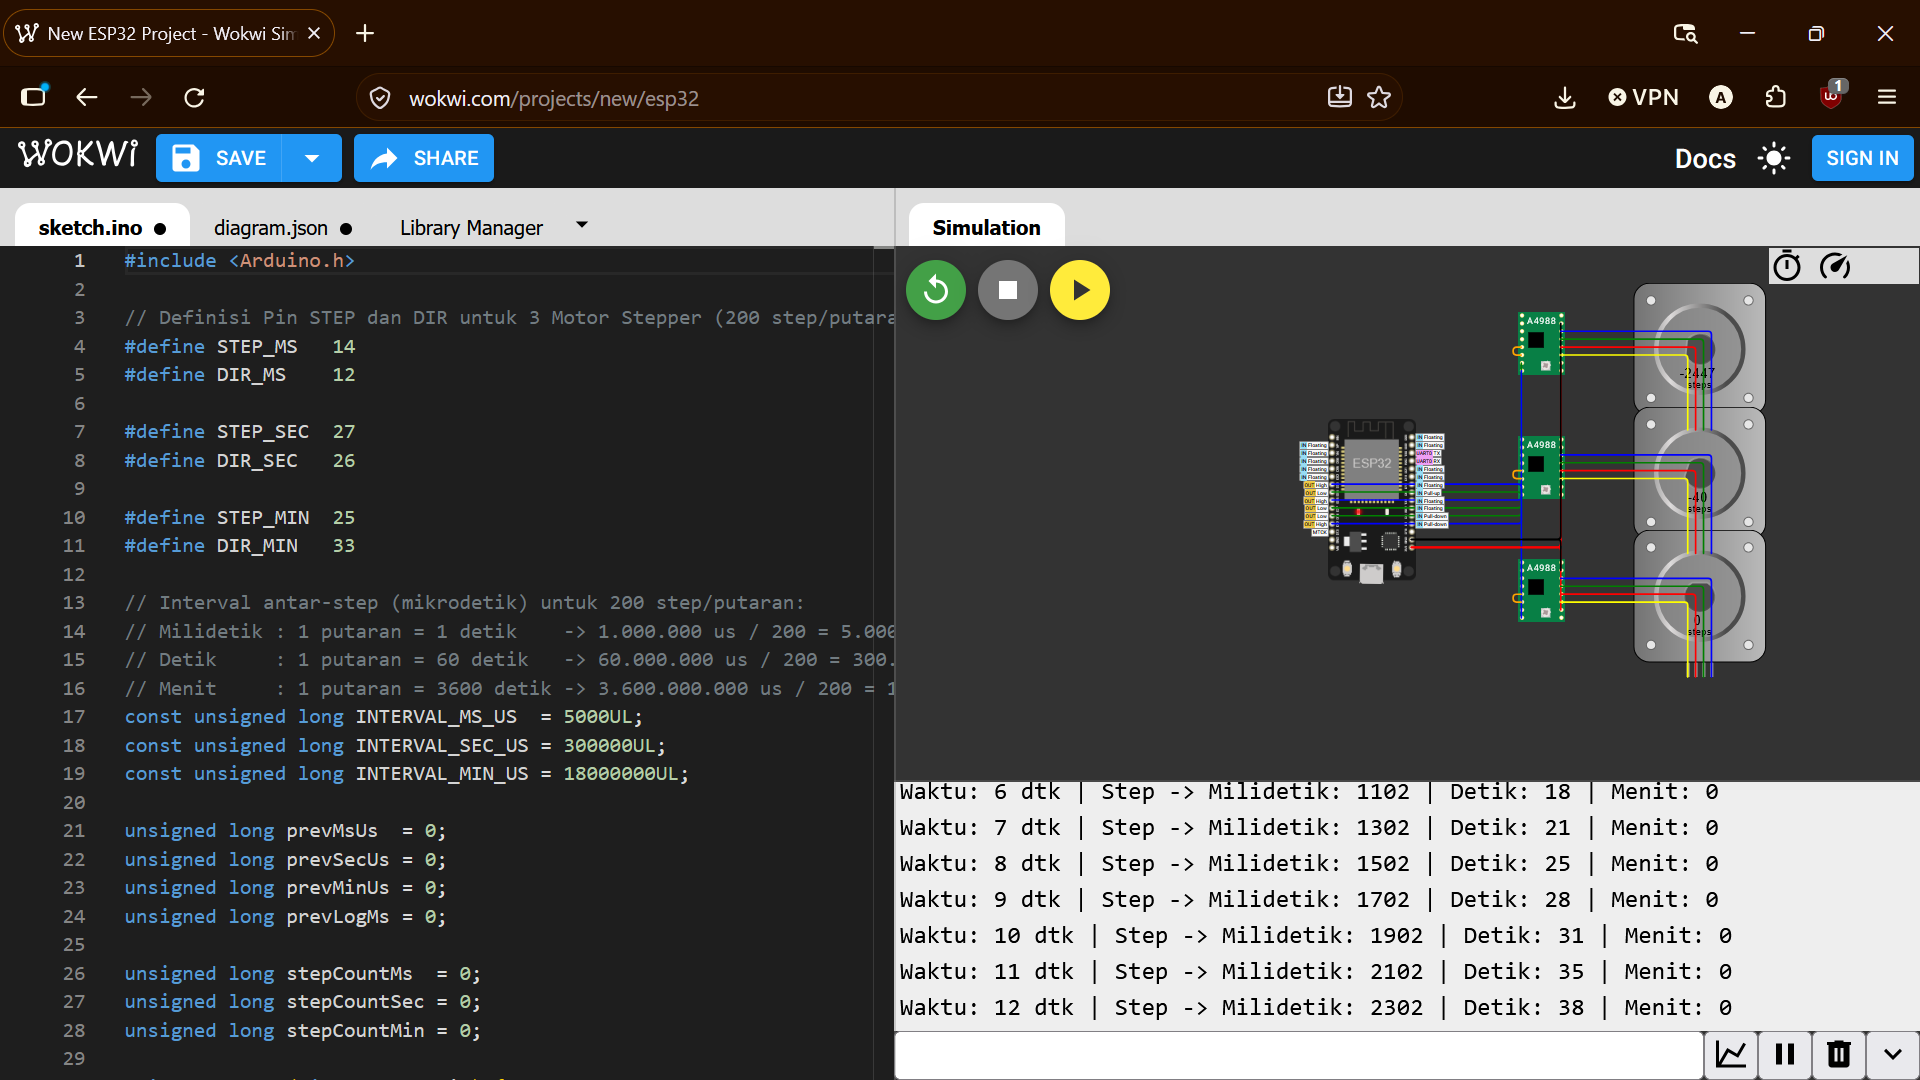
\includegraphics[width=0.85\textwidth]{tugas modul.png}
    \caption{Hasil simulasi ESP32 dengan tiga motor stepper sebagai jam analog (milidetik, detik, dan menit) pada Wokwi.}
    \label{fig:simulasi_jam_stepper}
\end{figure}

Berikut adalah kode program (\texttt{main.cpp}) yang digunakan dalam simulasi:

\begin{verbatim}
#include <Arduino.h>

#define STEP_MS   14
#define DIR_MS    12
#define STEP_SEC  27
#define DIR_SEC   26
#define STEP_MIN  25
#define DIR_MIN   33

// Interval antar-step (mikrodetik) untuk motor 200 step/putaran
const unsigned long INTERVAL_MS_US  = 5000UL;      // 60 RPM (1 putaran / 1 detik)
const unsigned long INTERVAL_SEC_US = 300000UL;    // 1 RPM (1 putaran / 60 detik)
const unsigned long INTERVAL_MIN_US = 18000000UL;  // 1/60 RPM (1 putaran / 3600 detik)

unsigned long prevMsUs = 0, prevSecUs = 0, prevMinUs = 0, prevLogMs = 0;
unsigned long stepCountMs = 0, stepCountSec = 0, stepCountMin = 0;

void pulseStep(uint8_t stepPin) {
  digitalWrite(stepPin, HIGH);
  delayMicroseconds(10);
  digitalWrite(stepPin, LOW);
}

void setup() {
  Serial.begin(115200);
  pinMode(STEP_MS, OUTPUT);  pinMode(DIR_MS, OUTPUT);
  pinMode(STEP_SEC, OUTPUT); pinMode(DIR_SEC, OUTPUT);
  pinMode(STEP_MIN, OUTPUT); pinMode(DIR_MIN, OUTPUT);

  // Arah putar searah jarum jam (CW)
  digitalWrite(DIR_MS, HIGH);
  digitalWrite(DIR_SEC, HIGH);
  digitalWrite(DIR_MIN, HIGH);

  unsigned long now = micros();
  prevMsUs = now; prevSecUs = now; prevMinUs = now;
}

void loop() {
  unsigned long nowUs = micros();

  if (nowUs - prevMsUs >= INTERVAL_MS_US) {
    prevMsUs += INTERVAL_MS_US;
    pulseStep(STEP_MS);
    stepCountMs++;
  }
  if (nowUs - prevSecUs >= INTERVAL_SEC_US) {
    prevSecUs += INTERVAL_SEC_US;
    pulseStep(STEP_SEC);
    stepCountSec++;
  }
  if (nowUs - prevMinUs >= INTERVAL_MIN_US) {
    prevMinUs += INTERVAL_MIN_US;
    pulseStep(STEP_MIN);
    stepCountMin++;
  }

  if (millis() - prevLogMs >= 1000) {
    prevLogMs += 1000;
    Serial.printf("Waktu: %lu dtk | Step -> Milidetik: %lu | Detik: %lu | Menit: %lu\n",
                  millis() / 1000, stepCountMs, stepCountSec, stepCountMin);
  }
}
\end{verbatim}

\subsection{Jawaban Pertanyaan Analisis}

\begin{enumerate}
    \item \textbf{Penentuan Kecepatan Putaran (RPM) dan STEP pada Masing-Masing Motor Stepper}

    Pada jam analog, setiap jarum menyelesaikan satu putaran penuh ($360^\circ$) dalam periode waktu yang berbeda. Dengan menggunakan motor stepper beresolusi $200$ step per putaran ($1,8^\circ$ per step), kecepatan putaran dalam satuan RPM (\textit{Revolution Per Minute}) serta jeda waktu antar-step ($\Delta t$) dihitung sebagai berikut:
    \begin{itemize}
        \item \textbf{Motor Milidetik (1 putaran penuh = 1 detik):} Jarum milidetik harus berputar penuh setiap $1$ detik ($1000$ ms), sehingga kecepatannya adalah
        \[
        \text{RPM}_{\text{ms}} = \frac{1\text{ putaran}}{1\text{ detik}} \times 60\text{ detik/menit} = 60\text{ RPM},
        \]
        dengan kebutuhan $200\text{ step/detik}$ dan jeda antar-step sebesar
        \[
        \Delta t_{\text{ms}} = \frac{1.000.000\ \mu\text{s}}{200\text{ step}} = 5.000\ \mu\text{s}.
        \]

        \item \textbf{Motor Detik (1 putaran penuh = 60 detik):} Jarum detik berputar penuh dalam $1$ menit ($60$ detik), sehingga kecepatannya adalah
        \[
        \text{RPM}_{\text{detik}} = \frac{1\text{ putaran}}{1\text{ menit}} = 1\text{ RPM},
        \]
        dengan laju sekitar $3,33\text{ step/detik}$ dan jeda antar-step sebesar
        \[
        \Delta t_{\text{detik}} = \frac{60.000.000\ \mu\text{s}}{200\text{ step}} = 300.000\ \mu\text{s}.
        \]

        \item \textbf{Motor Menit (1 putaran penuh = 3600 detik):} Jarum menit berputar penuh setiap $60$ menit ($3600$ detik), sehingga kecepatannya adalah
        \[
        \text{RPM}_{\text{menit}} = \frac{1\text{ putaran}}{60\text{ menit}} = \frac{1}{60}\text{ RPM} \approx 0,0167\text{ RPM},
        \]
        dengan laju sekitar $0,0556\text{ step/detik}$ dan jeda antar-step sebesar
        \[
        \Delta t_{\text{menit}} = \frac{3.600.000.000\ \mu\text{s}}{200\text{ step}} = 18.000.000\ \mu\text{s}.
        \]
    \end{itemize}
    Apabila motor yang digunakan adalah tipe 28BYJ-48 yang memiliki gearbox internal dengan resolusi $4096$ step per putaran, nilai RPM masing-masing jarum tetap sama, sedangkan pembagi pada perhitungan $\Delta t$ disesuaikan menjadi $4096$ step.

    \item \textbf{Kelayakan Penggantian Motor Stepper dengan Motor Servo}

    Motor stepper pada simulasi jam analog di atas \textbf{tidak dapat} digantikan dengan motor servo biasa karena dua keterbatasan berikut:
    \begin{itemize}
        \item \textbf{Batas Sudut Putaran ($0^\circ$--$180^\circ$):} Motor servo standar memiliki pembatas mekanis dan potensiometer internal yang membatasi geraknya hanya setengah lingkaran ($180^\circ$). Sebaliknya, jarum jam analog memerlukan putaran penuh $360^\circ$ secara terus-menerus tanpa harus berbalik arah mundur ketika mencapai batas sudut.
        \item \textbf{Presisi Langkah pada Servo Kontinu:} Meskipun tersedia jenis \textit{continuous rotation servo} yang mampu berputar $360^\circ$, sinyal PWM pada servo jenis ini hanya mengatur kecepatan dan arah putar layaknya motor DC, bukan posisi sudut diskret per langkah. Akibatnya, penunjukan posisi jarum jam mudah meleset seiring waktu tanpa sensor umpan balik tambahan seperti \textit{encoder}.
    \end{itemize}

    \item \textbf{Fungsi Driver Motor dan Alasan Penggunaannya pada Setiap Percobaan}

    Driver motor berperan sebagai perantara daya sekaligus penerjemah sinyal kontrol antara mikrokontroler (ESP32) dengan aktuator motor. Setiap motor dalam percobaan wajib menggunakan driver karena alasan berikut:
    \begin{itemize}
        \item \textbf{Penguatan Tegangan dan Arus:} Pin GPIO ESP32 hanya bekerja pada level logika $3,3$ V dengan arus keluaran sangat kecil (sekitar $12$--$40$ mA), sedangkan motor DC ($12$ V), motor stepper ($5$--$12$ V), dan motor BLDC ($7,4$--$11,1$ V) membutuhkan daya jauh lebih besar. Driver menyalurkan daya dari catu daya eksternal ke motor mengikuti sinyal logika rendah dari ESP32.
        \item \textbf{Pengaturan Polaritas, Urutan Fasa, dan Komutasi:} Driver mengubah sinyal digital ESP32 menjadi pola kerja yang sesuai untuk tiap motor, seperti membalik polaritas arah arus pada motor DC (L298N), mengatur urutan pengaktifan koil 4-fasa pada motor stepper (ULN2003 dan A4988), serta melakukan komutasi elektronik 3-fasa pada motor brushless (ESC).
        \item \textbf{Proteksi Rangkaian Mikrokontroler:} Driver memiliki rangkaian isolasi dan dioda \textit{flyback} untuk meredam lonjakan tegangan balik (\textit{back-EMF}) dari kumparan motor saat berputar atau berhenti mendadak agar pin ESP32 tidak rusak. Pada motor servo, rangkaian driver dan kontrol posisi tersebut sudah terpasang secara internal di dalam bodi motor.
    \end{itemize}
\end{enumerate}

\section{Kesimpulan}

Berdasarkan rangkaian percobaan dan simulasi pada \textbf{Modul 2: Sensor dan Aktuator Motor}, diperoleh beberapa kesimpulan utama sebagai berikut:

\begin{enumerate}
    \item \textbf{Integrasi Sensor sebagai Masukan Sistem:} Pembacaan data dari sensor (seperti sensor jarak ultrasonik maupun sensor lingkungan) oleh mikrokontroler ESP32 berjalan sesuai prinsip konversi besaran fisis menjadi sinyal elektrik. Data hasil pembacaan tersebut dapat diolah secara waktu nyata (\textit{real-time}) sebagai parameter pemicu maupun umpan balik dalam pengendalian aktuator.

    \item \textbf{Karakteristik dan Metode Kendali Aktuator Motor:} Setiap jenis motor memiliki karakteristik mekanis dan mekanisme kendali yang berbeda sesuai kebutuhan aplikasi sistem tertanam:
    \begin{itemize}
        \item \textbf{Motor DC:} Kecepatan putar diatur menggunakan modulasi lebar pulsa (\textit{Pulse Width Modulation}/PWM), sedangkan arah putaran ditentukan melalui pembalikan polaritas arus pada rangkaian \textit{H-Bridge}.
        \item \textbf{Motor Servo:} Pergerakan sudut dikendalikan secara diskret pada rentang terbatas ($0^\circ$--$180^\circ$) berdasarkan variasi lebar pulsa (\textit{duty cycle}) sinyal PWM dengan umpan balik potensiometer internal.
        \item \textbf{Motor Stepper:} Posisi sudut dan kecepatan putar dikendalikan secara presisi melalui cacah pulsa langkah (\texttt{STEP}) serta logika arah (\texttt{DIR}), sehingga mampu berputar $360^\circ$ secara kontinu tanpa memerlukan sensor posisi tambahan.
        \item \textbf{Motor BLDC:} Putaran motor dikendalikan melalui proses komutasi elektronik tiga fasa menggunakan \textit{Electronic Speed Controller} (ESC) yang menerima sinyal PWM dari mikrokontroler.
    \end{itemize}

    \item \textbf{Peran Vital Driver Motor:} Pin GPIO ESP32 bekerja pada level logika $3,3$ V dengan kapasitas arus terbatas, sehingga tidak mampu menggerakkan motor secara langsung. Penggunaan driver motor (seperti L298N, ULN2003, A4988, dan ESC) terbukti esensial sebagai penguat tegangan dan arus dari catu daya eksternal, penerjemah urutan fasa atau polaritas sinyal, sekaligus pelindung rangkaian mikrokontroler dari lonjakan tegangan balik (\textit{back-EMF}).

    \item \textbf{Sinkronisasi Pewaktuan Non-Blocking:} Pada simulasi jam analog berbasis tiga motor stepper, penggunaan pencacah waktu berbasis fungsi \texttt{micros()} dan \texttt{millis()} memungkinkan pembangkitan pulsa langkah berjalan secara bersamaan (\textit{concurrent}) pada kecepatan yang berbeda ($60$ RPM, $1$ RPM, dan $1/60$ RPM) tanpa saling menghambat eksekusi program utama.

    \item \textbf{Kesesuaian Hasil dengan Teori:} Seluruh hasil pengujian perangkat keras maupun simulasi pada Wokwi telah sesuai dengan teori dasar sensor dan aktuator. Pemilihan jenis motor dan driver dalam perancangan sistem tertanam harus disesuaikan dengan kebutuhan spesifik sistem, baik dari segi torsi, kecepatan putar, maupun ketelitian sudut gerak.
\end{enumerate}

\section{Lampiran}
\subsection{Dokumentasi saat praktikum}
% ==================== PERCOBAAN 1 ====================
\begin{figure}[H]
    \centering
    \includegraphics[width=0.75\textwidth]{"Merangkai.jpeg"}
    \caption{Proses Merangkai Komponen Percobaan 1}
    \label{fig:p1_merangkai}
\end{figure}

\begin{figure}[H]
    \centering
    \includegraphics[width=0.75\textwidth]{"Build upload.jpeg"}
    \caption{Proses Build dan Upload Program Percobaan 1}
    \label{fig:p1_build_upload}
\end{figure}

\begin{figure}[H]
    \centering
    \includegraphics[width=0.75\textwidth]{"Serial monitor touch sensor.jpeg"}
    \caption{Tampilan Serial Monitor Touch Sensor}
    \label{fig:p1_sm_touch}
\end{figure}

\begin{figure}[H]
    \centering
    \includegraphics[width=0.75\textwidth]{"Tes touch sensor.jpeg"}
    \caption{Pengujian Rangkaian Touch Sensor}
    \label{fig:p1_tes_touch}
\end{figure}

\begin{figure}[H]
    \centering
    \includegraphics[width=0.75\textwidth]{"Serial monitor joystick.jpeg"}
    \caption{Tampilan Awal Serial Monitor Joystick}
    \label{fig:p1_sm_joystick}
\end{figure}

\begin{figure}[H]
    \centering
    \includegraphics[width=0.75\textwidth]{"tes joystick atas.jpeg"}
    \caption{Pengujian Joystick Arah Atas}
    \label{fig:p1_tes_joystick_atas}
\end{figure}

\begin{figure}[H]
    \centering
    \includegraphics[width=0.75\textwidth]{"Tes joystick bawah.jpeg"}
    \caption{Pengujian Joystick Arah Bawah}
    \label{fig:p1_tes_joystick_bawah}
\end{figure}

\begin{figure}[H]
    \centering
    \includegraphics[width=0.75\textwidth]{"state zero joystick.jpeg"}
    \caption{Kondisi State Zero pada Joystick}
    \label{fig:p1_state_zero_joystick}
\end{figure}

\begin{figure}[H]
    \centering
    \includegraphics[width=0.75\textwidth]{"serial monitor joystick atas.jpeg"}
    \caption{Tampilan Serial Monitor Pengujian Joystick Atas}
    \label{fig:p1_sm_joystick_atas}
\end{figure}

\begin{figure}[H]
    \centering
    \includegraphics[width=0.75\textwidth]{"serial monitor joystick bawah.jpeg"}
    \caption{Tampilan Serial Monitor Pengujian Joystick Bawah}
    \label{fig:p1_sm_joystick_bawah}
\end{figure}

\begin{figure}[H]
    \centering
    \includegraphics[width=0.75\textwidth]{"hall effect state zero.jpeg"}
    \caption{Kondisi State Zero Sensor Hall Effect}
    \label{fig:p1_hall_state_zero}
\end{figure}

\begin{figure}[H]
    \centering
    \includegraphics[width=0.75\textwidth]{"rangkaian hall effect state zero.jpeg"}
    \caption{Rangkaian Sensor Hall Effect pada Kondisi State Zero}
    \label{fig:p1_rangkaian_hall_zero}
\end{figure}

\begin{figure}[H]
    \centering
    \includegraphics[width=0.75\textwidth]{"hall effect tes magnet.jpeg"}
    \caption{Pengujian Sensor Hall Effect dengan Magnet}
    \label{fig:p1_hall_tes_magnet}
\end{figure}

\begin{figure}[H]
    \centering
    \includegraphics[width=0.75\textwidth]{"serial monitor hall effect magnet.jpeg"}
    \caption{Tampilan Serial Monitor Sensor Hall Effect saat Didekatkan Magnet}
    \label{fig:p1_sm_hall_magnet}
\end{figure}

% ==================== PERCOBAAN 2 ====================
\begin{figure}[H]
    \centering
    \includegraphics[width=0.75\textwidth]{"srial monitor state zero.jpeg"}
    \caption{Tampilan Serial Monitor State Zero Percobaan 2}
    \label{fig:p2_sm_state_zero}
\end{figure}

\begin{figure}[H]
    \centering
    \includegraphics[width=0.75\textwidth]{"rangkaian state zero.jpeg"}
    \caption{Rangkaian Kondisi State Zero Percobaan 2}
    \label{fig:p2_rangkaian_state_zero}
\end{figure}

\begin{figure}[H]
    \centering
    \includegraphics[width=0.75\textwidth]{"rangkaian tes IR.jpeg"}
    \caption{Pengujian Rangkaian Sensor Inframerah (IR)}
    \label{fig:p2_rangkaian_tes_ir}
\end{figure}

\begin{figure}[H]
    \centering
    \includegraphics[width=0.75\textwidth]{"serial monitor tes IR.jpeg"}
    \caption{Tampilan Serial Monitor Pengujian Sensor Inframerah (IR)}
    \label{fig:p2_sm_tes_ir}
\end{figure}

\begin{figure}[H]
    \centering
    \includegraphics[width=0.75\textwidth]{"serial monitor ultrasonik state zero.jpeg"}
    \caption{Tampilan Serial Monitor Sensor Ultrasonik pada Kondisi State Zero}
    \label{fig:p2_sm_ultrasonik_zero}
\end{figure}

\begin{figure}[H]
    \centering
    \includegraphics[width=0.75\textwidth]{"tes ultrasonik.jpeg"}
    \caption{Pengujian Rangkaian Sensor Ultrasonik}
    \label{fig:p2_tes_ultrasonik}
\end{figure}

\begin{figure}[H]
    \centering
    \includegraphics[width=0.75\textwidth]{"serial monitor tes ultrasonik.jpeg"}
    \caption{Tampilan Serial Monitor Pengujian Sensor Ultrasonik}
    \label{fig:p2_sm_tes_ultrasonik}
\end{figure}

% ==================== PERCOBAAN 3 ====================
\begin{figure}[H]
    \centering
    \includegraphics[width=0.75\textwidth]{"rangkaian state zero.jpeg"}
    \caption{Rangkaian Kondisi State Zero Percobaan 3}
    \label{fig:p3_rangkaian_state_zero}
\end{figure}

\begin{figure}[H]
    \centering
    \includegraphics[width=0.75\textwidth]{"serialmonitor state zero.jpeg"}
    \caption{Tampilan Serial Monitor State Zero Percobaan 3}
    \label{fig:p3_sm_state_zero}
\end{figure}

\begin{figure}[H]
    \centering
    \includegraphics[width=0.75\textwidth]{"tes maju.jpeg"}
    \caption{Pengujian Gerak Maju Percobaan 3}
    \label{fig:p3_tes_maju}
\end{figure}

\begin{figure}[H]
    \centering
    \includegraphics[width=0.75\textwidth]{"serial monitor tes maju.jpeg"}
    \caption{Tampilan Serial Monitor Pengujian Gerak Maju}
    \label{fig:p3_sm_tes_maju}
\end{figure}

\begin{figure}[H]
    \centering
    \includegraphics[width=0.75\textwidth]{"tes mundur.jpeg"}
    \caption{Pengujian Gerak Mundur Percobaan 3}
    \label{fig:p3_tes_mundur}
\end{figure}

\begin{figure}[H]
    \centering
    \includegraphics[width=0.75\textwidth]{"serial monitor mundur.jpeg"}
    \caption{Tampilan Serial Monitor Pengujian Gerak Mundur}
    \label{fig:p3_sm_mundur}
\end{figure}

\begin{figure}[H]
    \centering
    \includegraphics[width=0.75\textwidth]{"rangkaian tes putar.jpeg"}
    \caption{Pengujian Rangkaian Putar Percobaan 3}
    \label{fig:p3_rangkaian_tes_putar}
\end{figure}

% ==================== PERCOBAAN 4 ====================
\begin{figure}[H]
    \centering
    \includegraphics[width=0.75\textwidth]{"rangkaian state zero.jpeg"}
    \caption{Rangkaian Kondisi State Zero Percobaan 4}
    \label{fig:p4_rangkaian_state_zero}
\end{figure}

\begin{figure}[H]
    \centering
    \includegraphics[width=0.75\textwidth]{"serial monitor setelah upload.jpeg"}
    \caption{Tampilan Serial Monitor Setelah Upload Program Percobaan 4}
    \label{fig:p4_sm_setelah_upload}
\end{figure}

\begin{figure}[H]
    \centering
    \includegraphics[width=0.75\textwidth]{"tes putar 1.jpeg"}
    \caption{Pengujian Putar Tahap 1 Percobaan 4}
    \label{fig:p4_tes_putar_1}
\end{figure}

\begin{figure}[H]
    \centering
    \includegraphics[width=0.75\textwidth]{"tes putar 2.jpeg"}
    \caption{Pengujian Putar Tahap 2 Percobaan 4}
    \label{fig:p4_tes_putar_2}
\end{figure}

% ==================== PERCOBAAN 5 ====================
\begin{figure}[H]
    \centering
    \includegraphics[width=0.75\textwidth]{"serial monitor state zero.jpeg"}
    \caption{Tampilan Serial Monitor State Zero Percobaan 5}
    \label{fig:p5_sm_state_zero}
\end{figure}

\begin{figure}[H]
    \centering
    \includegraphics[width=0.75\textwidth]{"rangkaian tes putar 1.jpeg"}
    \caption{Pengujian Rangkaian Putar Tahap 1 Percobaan 5}
    \label{fig:p5_rangkaian_tes_putar_1}
\end{figure}

\begin{figure}[H]
    \centering
    \includegraphics[width=0.75\textwidth]{"rangkaian tes putar 2.jpeg"}
    \caption{Pengujian Rangkaian Putar Tahap 2 Percobaan 5}
    \label{fig:p5_rangkaian_tes_putar_2}
\end{figure}

% ==================== PERCOBAAN 6 ====================
\begin{figure}[H]
    \centering
    \includegraphics[width=0.75\textwidth]{"rangkaian setelah upload.jpeg"}
    \caption{Rangkaian Setelah Proses Upload Program Percobaan 6}
    \label{fig:p6_rangkaian_setelah_upload}
\end{figure}

\begin{figure}[H]
    \centering
    \includegraphics[width=0.75\textwidth]{"motor berputar sesuai program.jpeg"}
    \caption{Kondisi Motor Berputar Sesuai Program}
    \label{fig:p6_motor_berputar}
\end{figure}

\begin{figure}[H]
    \centering
    \includegraphics[width=0.75\textwidth]{"motor berhenti sesuai program.jpeg"}
    \caption{Kondisi Motor Berhenti Sesuai Program}
    \label{fig:p6_motor_berhenti}
\end{figure}